
\begin{frame}{What is artificial intelligence?}
    \begin{tikzpicture}

        \node[] at (-7, -3.25) {};
        \node[] at (7, 3.25) {};

        \only<1>{
            \node[anchor=west, inner sep=0pt, draw=black, label=below:\tiny{ChatGPT}] at (-7, 0) {
                
\includegraphics[width=4.1cm]{data/chatgpt.png}
            };
            \node[inner sep=0pt, draw=black, label=below:\tiny{Spot}] at (-0.5, 1.5) {
                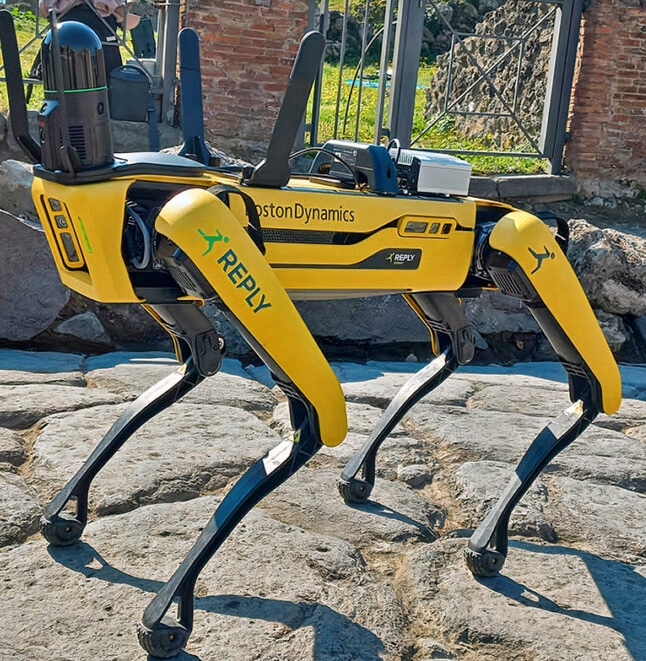
\includegraphics[width=3cm]{data/spot.jpg}
            };
            \node[inner sep=0pt, draw=black, label=below:\tiny{Sophia}] at (2.7, 1.5) {
                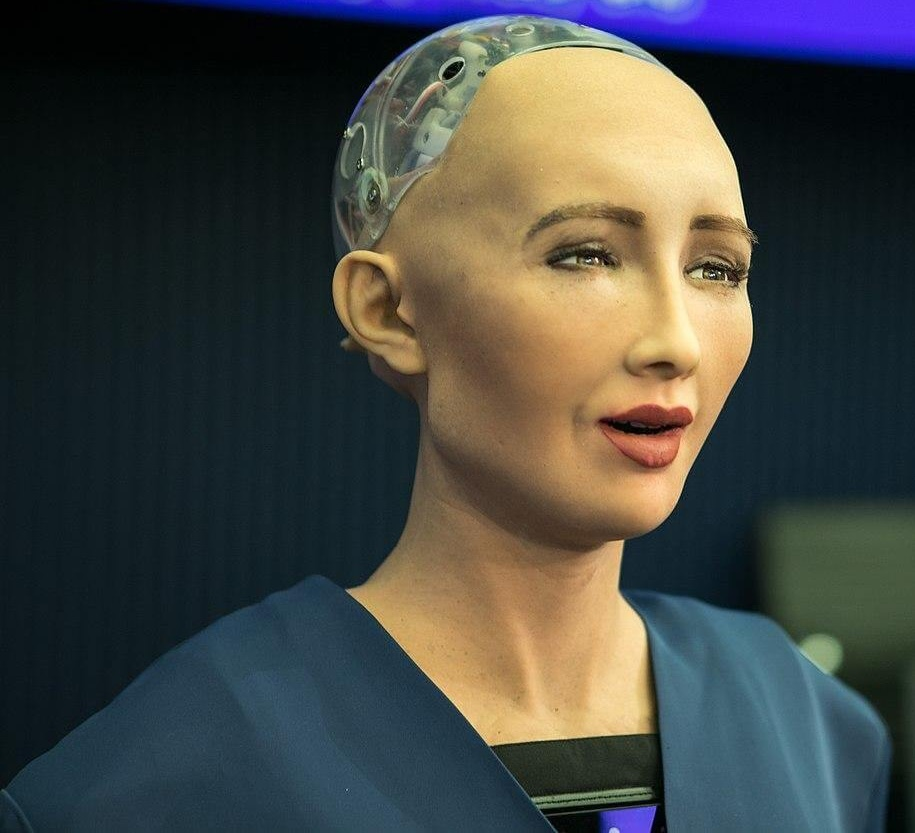
\includegraphics[width=3cm]{data/sophia.jpg}
            };
            \node[inner sep=0pt, draw=black, label=below:\tiny{AlphaFold}] at (1, -1.5) {
                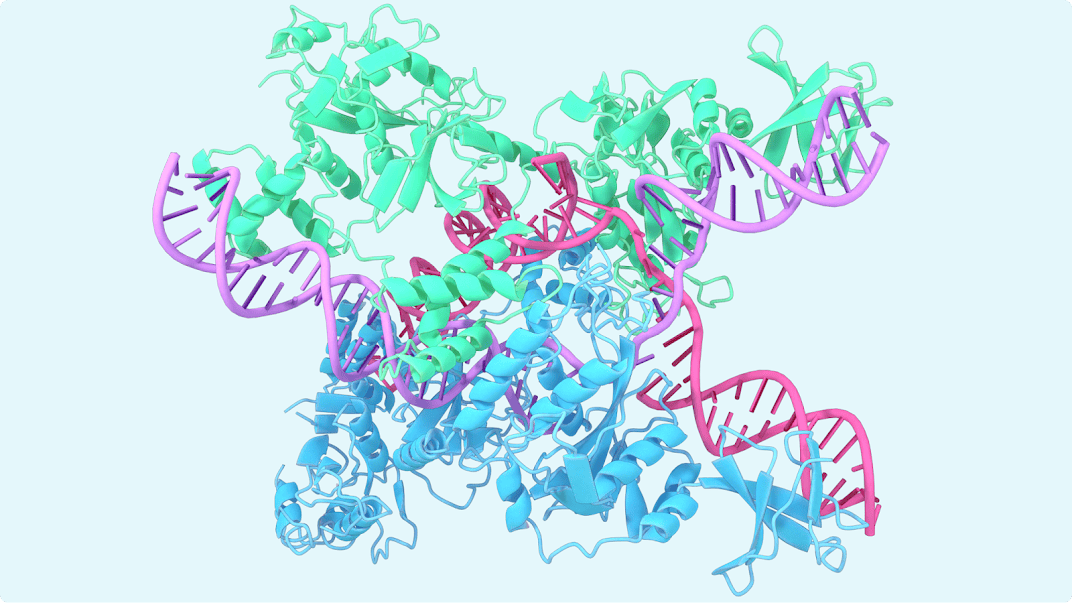
\includegraphics[width=4cm]{data/alphafold.png}
            };
        }

        \only<2-4,9,13-14,18>{
            \node[circle, fill=uioblue!80, minimum size=6cm, anchor=north] (ai) at (-4, 3.25) {};
            \node[white, anchor=north, align=center, font=\small\bfseries\linespread{0.9}\selectfont] at ($ (ai.north) - (0, 0.1) $) {Artificial\\intelligence};

            \only<2>{
                \node[align=flush left, anchor=north west, text width=7.2cm, font=\small\linespread{0.95}\selectfont] (def1) at (-0.5, 3.25) {
                    \textbf{Artificial intelligence}\\
                    Technology that solves tasks requiring some form of intelligence
                };
            }
            \only<3->{
                \node[align=flush left, anchor=north west, text width=7.2cm, font=\small\linespread{0.95}\selectfont] (def1) at (-0.5, 3.25) {
                    \textbf{Artificial intelligence}\\
                    The field of study producing technology that solves tasks requiring some form of intelligence
                };
            }

            \only<4->{
                \node[align=center, font=\small\linespread{0.9}\selectfont, text=white] at ($ (ai.north) + (1.3, -1.5) $) {Rule-based\\systems};
            }

            \only<9->{
                \node[circle, fill=uioblue!50!uiored!80, anchor=south, minimum size=4.1cm] (ml) at ($ (ai.south) + (0, 0.05) $) {};
                \node[white, anchor=north, align=center, font=\small\bfseries\linespread{0.9}\selectfont] at ($ (ml.north) - (0, 0.1) $) {Machine\\learning};
            }
            \only<13->{
                \node[align=flush left, anchor=north west, text width=7.2cm, font=\small\linespread{0.95}\selectfont] (def2) at (def1.south west) {
                    \textbf{Machine learning}\\
                    Technologies that learn to solve problems by finding patterns in training data
                };
            }
            \only<14->{
                \node[circle, fill=uiored!80, anchor=south, minimum size=3cm] (dl) at ($ (ml.south) + (0, 0.06) $) {};
                \node[white, anchor=north, align=center, font=\small\bfseries\linespread{0.9}\selectfont] at ($ (dl.north) - (0, 0.1) $) {Deep\\learning};
            }
            \only<18>{
                \node[align=flush left, anchor=north west, text width=7.2cm, font=\small\linespread{0.95}\selectfont] (def3) at (def2.south west) {
                \textbf{Deep learning}\\
                    Technologies that rely on artificial neural networks to solve machine learning problems
                };
            }
        }
        \only<5-8>{
            \node[draw=black, fill=gray!90, minimum width=6cm, minimum height=3.5cm, rounded corners=0.1cm, text=white, text depth=3cm, font=\systemfont] (system) at (0, 1) {Expert system};

            \only<6->{
                \node[draw=black, label=below:\systemfont{Prediction}, anchor=west] (output) at ($ (system.south east) + (1, 1.3) $) {
                    \systemfont{Influenza}
                };

                \node[] (notepad) at ($ (system.south west) + (-1, 1.3) $) {\Large{\emoji{spiral-notepad}}};
                \node[anchor=east, inner sep=-2pt] at (notepad.west) {\Huge{\emoji{man-health-worker}}};

                \draw[-stealth] (notepad.east) -- ($ (system.south west) + (0, 1.3) $);
                \draw[-stealth] ($ (system.south east) + (0, 1.3) $) -- (output);
            }

            \only<7->{
                \node[fill=gray!80, minimum width=4cm, minimum height=2.9cm, rounded corners=0.1cm, text=white, draw=black, font=\systemfont, anchor=south, text depth=2.4cm] (rule) at ($ (system.south) + (0, 0.05) $) {
                    Rule engine
                };
                \node[draw=black, fill=white, rounded corners=0.05cm, font=\systemfont, minimum width=1.9cm, minimum height=0.55cm] (symptom1) at ($ (rule.south) + (0, 1.95) $) {Fever};
                \node[draw=black, fill=white, rounded corners=0.05cm, font=\systemfont, minimum width=1.9cm, minimum height=0.55cm] (symptom2) at ($ (rule.south) + (0, 1.25) $) {Cough};
                \node[draw=black, fill=white, rounded corners=0.05cm, font=\systemfont, minimum width=1.9cm, minimum height=0.55cm] (symptom3) at ($ (rule.south) + (0, 0.55) $) {Sore throat};

                \draw[-stealth] ($ (system.south west) + (0, 1.3) $) -- ($ (rule.south west) + (0, 1.25) $);
                \draw[-stealth] ($ (rule.south west) + (0, 1.25) $) -- (symptom1.west);
                \draw[-stealth] ($ (rule.south west) + (0, 1.25) $) -- (symptom2.west);
                \draw[-stealth] ($ (rule.south west) + (0, 1.25) $) -- (symptom3.west);
                \draw[-stealth] (symptom1.east) -- ($ (rule.south east) + (0, 1.25) $);
                \draw[-stealth] (symptom2.east) -- ($ (rule.south east) + (0, 1.25) $);
                \draw[-stealth] (symptom3.east) -- ($ (rule.south east) + (0, 1.25) $);
                \draw[-stealth] ($ (rule.south east) + (0, 1.25) $) -- ($ (system.south east) + (0, 1.3) $);
            }
            \only<8>{
                \node[] (expert) at ($ (system.south) - (0, 1.75) $) {
                    \Huge{\emoji{woman-scientist}}
                };
                \draw[-stealth, dashed] (expert) -- (rule.south);
            }
        }
        \only<10-12>{
            \only<10>{
                \node[draw=black, fill=gray!90, minimum width=6cm, minimum height=3.5cm, rounded corners=0.1cm, text=white, text depth=3cm, font=\systemfont] (system) at (0, 1) {Expert system};
                \node[fill=gray!80, minimum width=4cm, minimum height=2.9cm, rounded corners=0.1cm, text=white, draw=black, font=\systemfont, anchor=south, text depth=2.4cm] (rule) at ($ (system.south) + (0, 0.05) $) {
                    Rule engine
                };
                \node[draw=black, fill=white, rounded corners=0.05cm, font=\systemfont, minimum width=1.9cm, minimum height=0.55cm] (symptom1) at ($ (rule.south) + (0, 1.95) $) {Fever};
                \node[draw=black, fill=white, rounded corners=0.05cm, font=\systemfont, minimum width=1.9cm, minimum height=0.55cm] (symptom2) at ($ (rule.south) + (0, 1.25) $) {Cough};
                \node[draw=black, fill=white, rounded corners=0.05cm, font=\systemfont, minimum width=1.9cm, minimum height=0.55cm] (symptom3) at ($ (rule.south) + (0, 0.55) $) {Sore throat};

                \draw[-stealth] ($ (system.south west) + (0, 1.3) $) -- ($ (rule.south west) + (0, 1.25) $);
                \draw[-stealth] ($ (rule.south west) + (0, 1.25) $) -- (symptom1.west);
                \draw[-stealth] ($ (rule.south west) + (0, 1.25) $) -- (symptom2.west);
                \draw[-stealth] ($ (rule.south west) + (0, 1.25) $) -- (symptom3.west);
                \draw[-stealth] (symptom1.east) -- ($ (rule.south east) + (0, 1.25) $);
                \draw[-stealth] (symptom2.east) -- ($ (rule.south east) + (0, 1.25) $);
                \draw[-stealth] (symptom3.east) -- ($ (rule.south east) + (0, 1.25) $);
                \draw[-stealth] ($ (rule.south east) + (0, 1.25) $) -- ($ (system.south east) + (0, 1.3) $);

                \node[] (expert) at ($ (system.south) - (0, 1.75) $) {
                    \Huge{\emoji{woman-scientist}}
                };
                \draw[-stealth, dashed] (expert) -- (rule.south);
            }
            \only<11->{
                \node[draw=black, fill=gray!90, minimum width=6cm, minimum height=3.5cm, rounded corners=0.1cm, text=white, text depth=3cm, font=\systemfont] (system) at (0, 1) {Machine learning system};
                \node[fill=gray!80, minimum width=4cm, minimum height=2.9cm, rounded corners=0.1cm, text=white, draw=black, font=\systemfont, anchor=south, text depth=2.4cm] (rule) at ($ (system.south) + (0, 0.05) $) {
                    Machine learning model
                };

                \node[] at ($ (rule.south) + (0, 1.25) $) {
                    
\includegraphics[width=3.75cm]{data/cogwheels.png}
                };

                \draw[-stealth] ($ (system.south west) + (0, 1.3) $) -- ($ (rule.south west) + (0, 1.25) $);
                \draw[-stealth] ($ (rule.south east) + (0, 1.25) $) -- ($ (system.south east) + (0, 1.3) $);
            }
            \only<12>{
                \node[] (expert) at ($ (system.south) - (0, 1.75) $) {
                    \Huge{\emoji{bar-chart}}
                };
                \draw[-stealth, dashed] (expert) -- (rule.south);
            }

            \node[draw=black, label=below:\systemfont{Prediction}, anchor=west] (output) at ($ (system.south east) + (1, 1.3) $) {
                \systemfont{Influenza}
            };

            \node[] (notepad) at ($ (system.south west) + (-1, 1.3) $) {\Large{\emoji{spiral-notepad}}};
            \node[anchor=east, inner sep=-2pt] at (notepad.west) {\Huge{\emoji{man-health-worker}}};

            \draw[-stealth] (notepad.east) -- ($ (system.south west) + (0, 1.3) $);
            \draw[-stealth] ($ (system.south east) + (0, 1.3) $) -- (output);
        }
        \only<15-17>{
            \node[draw=black, fill=gray!90, minimum width=6cm, minimum height=3.5cm, rounded corners=0.1cm, text=white, text depth=3cm, font=\systemfont] (system) at (0, 1) {Machine learning system};
            \node[fill=gray!80, minimum width=4cm, minimum height=2.9cm, rounded corners=0.1cm, text=white, draw=black, font=\systemfont, anchor=south, text depth=2.4cm] (rule) at ($ (system.south) + (0, 0.05) $) {
                \only<15>{
                    Machine learning model
                }
                \only<16->{
                    Artificial neural network
                }
            };

            \only<15>{
                \node[] at ($ (rule.south) + (0, 1.25) $) {
                    
\includegraphics[width=3.75cm]{data/cogwheels.png}
                };
            }

            \only<16->{
                \neuron{n00}{($ (rule.south) + (0, 1.25) + (-2*\hsep, -2*\vsep) $)}
                \neuron{n01}{($ (n00) + (0, \vsep) $)}
                \neuron{n02}{($ (n00) + (0, 2*\vsep) $)}
                \neuron{n03}{($ (n00) + (0, 3*\vsep) $)}
                \neuron{n04}{($ (n00) + (0, 4*\vsep) $)}

                \neuron{n10}{($ (n00) + (\hsep, 0.5*\vsep) $)}
                \neuron{n11}{($ (n00) + (\hsep, 1.5*\vsep) $)}
                \neuron{n12}{($ (n00) + (\hsep, 2.5*\vsep) $)}
                \neuron{n13}{($ (n00) + (\hsep, 3.5*\vsep) $)}

                \neuron{n20}{($ (n00) + (2*\hsep, \vsep) $)}
                \neuron{n21}{($ (n00) + (2*\hsep, 2*\vsep) $)}
                \neuron{n22}{($ (n00) + (2*\hsep, 3*\vsep) $)}

                \neuron{n30}{($ (n00) + (3*\hsep, 1.5*\vsep) $)}
                \neuron{n31}{($ (n00) + (3*\hsep, 2.5*\vsep) $)}

                \neuron{n40}{($ (n00) + (4*\hsep, 2*\vsep) $)}

                \foreach \j in {0,...,4} {
                    \draw[black, opacity=\edgeopacity] ($ (rule.west) - (0, 0.2175) $) -- (n0\j);
                }

                \foreach \j in {0,...,4} {
                    \foreach \k in {0,...,3} {
                        \draw[black, opacity=\edgeopacity] (n0\j) -- (n1\k);
                    }
                }
                \foreach \j in {0,...,3} {
                    \foreach \k in {0,...,2} {
                        \draw[black, opacity=\edgeopacity] (n1\j) -- (n2\k);
                    }
                }
                \foreach \j in {0,...,2} {
                    \foreach \k in {0,...,1} {
                        \draw[black, opacity=\edgeopacity] (n2\j) -- (n3\k);
                    }
                }
                \draw[black, opacity=\edgeopacity] (n30) -- (n40);
                \draw[black, opacity=\edgeopacity] (n31) -- (n40);
                \draw[black, opacity=\edgeopacity] (n40) -- ($ (rule.south east) + (0, 1.25) $);
            }


            \draw[-stealth] ($ (system.south west) + (0, 1.3) $) -- ($ (rule.south west) + (0, 1.25) $);

            \draw[-stealth] ($ (rule.south east) + (0, 1.25) $) -- ($ (system.south east) + (0, 1.3) $);

            \only<15-16>{
                \node[] (expert) at ($ (system.south) - (0, 1.75) $) {
                    \Huge{\emoji{bar-chart}}
                };
                \draw[-stealth, dashed] (expert) -- (rule.south);
            }
            \only<17>{
                \node[circle, draw=black, fill=uiolightblue, minimum size=0.5cm] (neuron) at ($ (system.south) - (0, 1.1) $) {};

                \node[anchor=east, font=\scriptsize] (x1) at ($ (neuron) - (0.75, -0.5) $) {$\text{input}_1$};
                \node[anchor=east, font=\scriptsize] (x2) at ($ (neuron) - (0.75, 0) $) {$\text{input}_2$};
                \node[anchor=east, font=\scriptsize] (x3) at ($ (neuron) - (0.75, 0.5) $) {$\text{input}_3$};

                \node[anchor=west, font=\scriptsize] (y) at ($ (neuron) + (0.75, 0) $) {$\text{output}$};

                \draw[-stealth] (x1) -- (neuron);
                \draw[-stealth] (x2) -- (neuron);
                \draw[-stealth] (x3) -- (neuron);
                \draw[-stealth] (neuron) -- (y);

                \node[font=\small] at ($ (neuron) - (0, 1.1) $) {
                    Artificial neuron
                };
            }

            \node[draw=black, label=below:\systemfont{Prediction}, anchor=west] (output) at ($ (system.south east) + (1, 1.3) $) {
                \systemfont{Influenza}
            };

            \node[] (notepad) at ($ (system.south west) + (-1, 1.3) $) {\Large{\emoji{spiral-notepad}}};
            \node[anchor=east, inner sep=-2pt] at (notepad.west) {\Huge{\emoji{man-health-worker}}};

            \draw[-stealth] (notepad.east) -- ($ (system.south west) + (0, 1.3) $);
            \draw[-stealth] ($ (system.south east) + (0, 1.3) $) -- (output);
        }
    \end{tikzpicture}
\end{frame}

\begin{frame}{Why do we use artificial neural networks?}
    \begin{tikzpicture}
        \node[] at (-7, -3.25) {};
        \node[] at (7, 3.25) {};

        \visible<1-4>{
            \node[anchor=east] (input) at (-3, 1.25) {$\text{input}$};
            \node[anchor=west] (output) at (3, 1.25) {$\text{output}$};
        }
        \visible<5>{
            \node[anchor=east, inner sep=0pt, draw=black] (input) at (-3, 1.25) {
                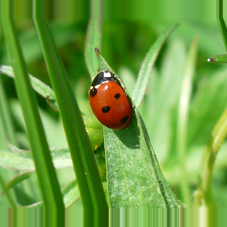
\includegraphics[width=2.5cm]{data/ladybug.png}
            };
            \node[anchor=west] (output) at (3, 1.25) {$\text{ladybug}$};
        }

        \visible<1-2,4-5>{
            \node[fill=gray!80, minimum width=4cm, minimum height=2.9cm, rounded corners=0.1cm, text=white, draw=black, font=\systemfont, anchor=south, text depth=2.4cm] (rule) at (0, 0) {
                Artificial neural network
            };
            \draw[-stealth] (input) -- ($ (rule.south west) + (0, 1.25) $);
            \draw[-stealth] ($ (rule.south east) + (0, 1.25) $) -- (output);
            \neuron{n00}{($ (rule.south) + (0, 1.25) + (-2*\hsep, -2*\vsep) $)}
            \neuron{n01}{($ (n00) + (0, \vsep) $)}
            \neuron{n02}{($ (n00) + (0, 2*\vsep) $)}
            \neuron{n03}{($ (n00) + (0, 3*\vsep) $)}
            \neuron{n04}{($ (n00) + (0, 4*\vsep) $)}

            \neuron{n10}{($ (n00) + (\hsep, 0.5*\vsep) $)}
            \neuron{n11}{($ (n00) + (\hsep, 1.5*\vsep) $)}
            \neuron{n12}{($ (n00) + (\hsep, 2.5*\vsep) $)}
            \neuron{n13}{($ (n00) + (\hsep, 3.5*\vsep) $)}

            \neuron{n20}{($ (n00) + (2*\hsep, \vsep) $)}
            \neuron{n21}{($ (n00) + (2*\hsep, 2*\vsep) $)}
            \neuron{n22}{($ (n00) + (2*\hsep, 3*\vsep) $)}

            \neuron{n30}{($ (n00) + (3*\hsep, 1.5*\vsep) $)}
            \neuron{n31}{($ (n00) + (3*\hsep, 2.5*\vsep) $)}

            \neuron{n40}{($ (n00) + (4*\hsep, 2*\vsep) $)}

            \foreach \j in {0,...,4} {
                \draw[black, opacity=\edgeopacity] ($ (rule.west) - (0, 0.2175) $) -- (n0\j);
            }

            \foreach \j in {0,...,4} {
                \foreach \k in {0,...,3} {
                    \draw[black, opacity=\edgeopacity] (n0\j) -- (n1\k);
                }
            }
            \foreach \j in {0,...,3} {
                \foreach \k in {0,...,2} {
                    \draw[black, opacity=\edgeopacity] (n1\j) -- (n2\k);
                }
            }
            \foreach \j in {0,...,2} {
                \foreach \k in {0,...,1} {
                    \draw[black, opacity=\edgeopacity] (n2\j) -- (n3\k);
                }
            }
            \draw[black, opacity=\edgeopacity] (n30) -- (n40);
            \draw[black, opacity=\edgeopacity] (n31) -- (n40);
            \draw[black, opacity=\edgeopacity] (n40) -- ($ (rule.south east) + (0, 1.25) $);
        }

        \visible<3>{
            \neuron{neuron}{($ (rule.south) + (0, 1.25) $)}
            \draw[-stealth] (input) -- (neuron);
            \draw[-stealth] (neuron) -- (output);
        }
    \end{tikzpicture}
\end{frame}